\begin{exo}
  \donnee{Un système électronique est formé des composants A, B, C et D placés selon le dispositif de la Figure 1. On suppose que les composants fonctionnent indépendamment les uns des autres et leurs probabilités de fonctionnement sont toutes égales à 0.8. Le système est opérationnel s’il existe un chemin entre les points I et O ne comprenant que des composants qui fonctionnent. Calculer la probabilité que le système soit défaillant.\\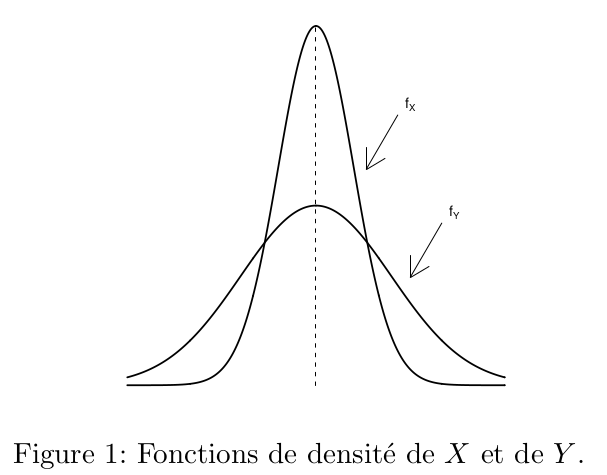
\includegraphics[width=10cm]{ex5.png}}
  \begin{flushleft}
    Prenons $A$ = "A fonctionne" et $\conj{A}$ ="A ne fonctionne pas". Pour que le système soit défaillant, il faut que la partie du bas et la partie du haut soit disfonctionnelle simultanément. Pour que la partie du haut soit disfonctionnelle il faut que soit A soit (B et C) ne fonctionnent pas ce qui se traduit par $\conj{A} \cup (\conj{B}\cap \conj{C})$. Donc la probabilité pour que le système soit défaillant: $P\Big(\conj{D}\cap \big( \conj{A} \cup (\conj{B}\cap \conj{C})\big)\Big)$
    \begin{align*}
    \\P(\conj{A} \cup (\conj{B} \cap \conj{C}))
    &= P(\conj{A}) + P(\conj{B} \cap \conj{C}) - P(\conj{A} \cap (\conj{B} \cap \conj{C})
    \\&= P(\conj{A}) + P(\conj{B})P(\conj{C}) -  P(\conj{A})\cdot P(\conj{B})P(\conj{C})
    \\&= P(\conj{A}) + P(\conj{B})P(\conj{C}) \cdot \big(1-P(\conj{A})\big)
    \\&= 0,2 + 0,04 \cdot 0,8 = 0,232
    \end{align*}
    \\ Alors
    \\$P\Big(\conj{D}\cap \big( \conj{A} \cup (\conj{B}\cap \conj{C})\big)\Big) = P(\conj{D})\cdot P(\conj{A} \cup (\conj{B} \cap \conj{C})) = 0,2 \cdot 0,232  = 0,0464$
  \end{flushleft}
\end{exo}
